% MV-Align Framework - 完整数据流架构图
\documentclass[tikz,border=6pt]{standalone}
\usepackage{amsmath}
\usepackage{tikz}
\usetikzlibrary{positioning, arrows.meta, backgrounds, fit}

% 配色
\definecolor{rawtext}{RGB}{255,248,220}
\definecolor{idblue}{RGB}{173,216,230}
\definecolor{tfidf}{RGB}{255,228,196}
\definecolor{llm}{RGB}{204,238,214}
\definecolor{v1}{RGB}{255,200,210}
\definecolor{v2}{RGB}{230,200,240}
\definecolor{v3}{RGB}{200,230,240}
\definecolor{v4}{RGB}{255,240,215}
\definecolor{align}{RGB}{255,255,224}

\tikzset{
  raw/.style={rectangle, rounded corners=1pt, draw=black!40, line width=0.6pt,
              minimum height=0.4cm, font=\scriptsize\sffamily, fill=rawtext},
  feat/.style={rectangle, rounded corners=2pt, draw=black, line width=0.9pt,
               minimum height=0.48cm, font=\small\sffamily},
  proc/.style={rectangle, draw=black!60, line width=0.7pt,
               minimum height=0.4cm, font=\footnotesize\sffamily, fill=white},
  small/.style={rectangle, draw=black!60, line width=0.6pt,
                minimum height=0.36cm, font=\scriptsize\sffamily, fill=white},
  arr/.style={-Stealth, line width=0.9pt},
  darr/.style={-Stealth, line width=0.7pt, dashed, color=orange!70},
}

\begin{document}
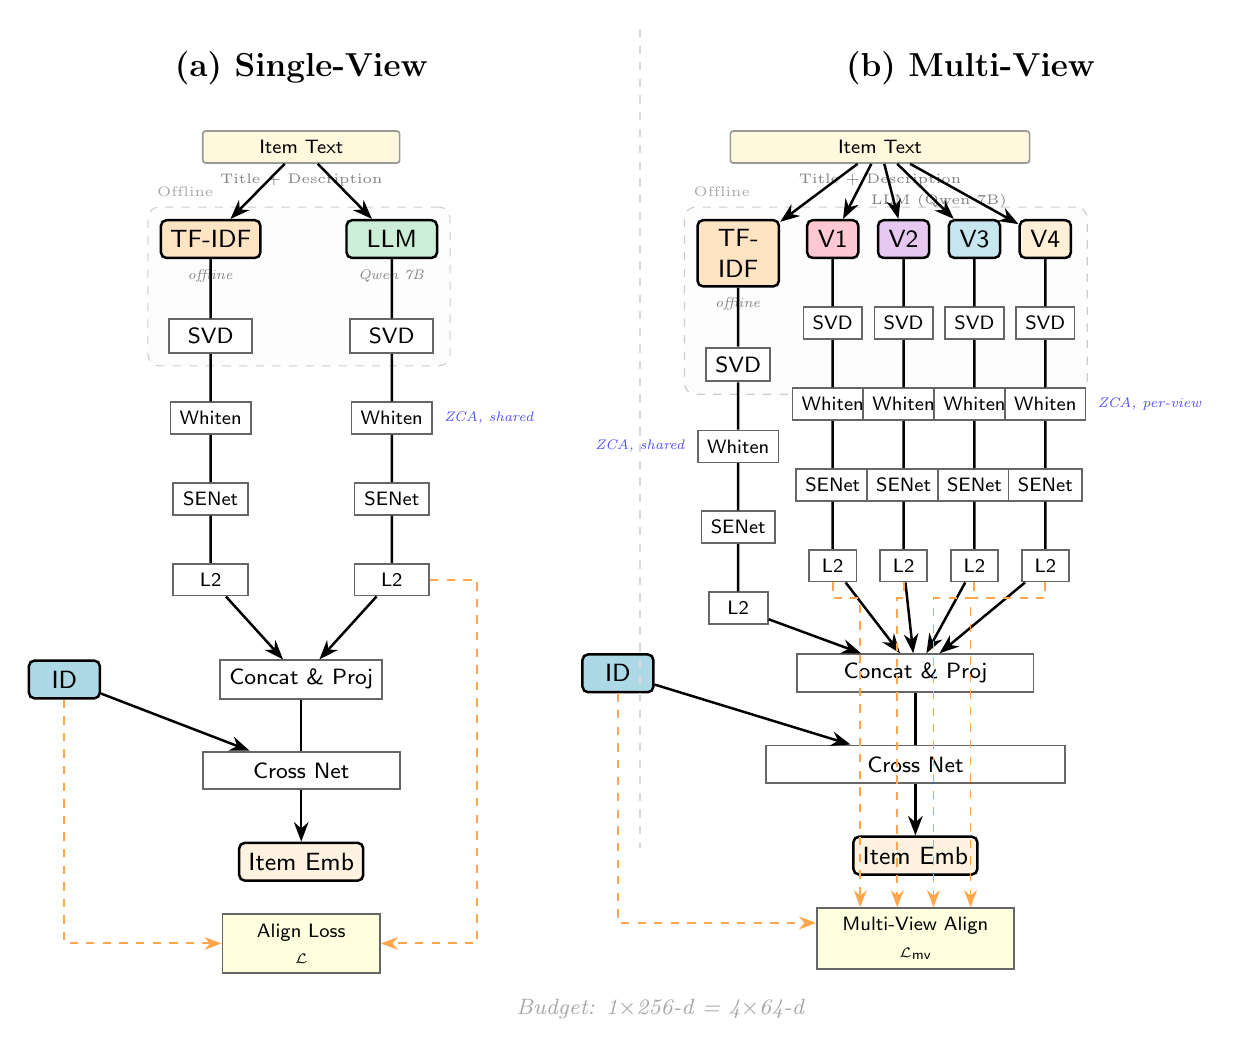
\begin{tikzpicture}[node distance=0.65cm]

% ========== Titles ==========
\node[font=\large\bfseries] at (-1.5, 0.6) {(a) Single-View};
\node[font=\large\bfseries] at (7, 0.6) {(b) Multi-View};

% ==================== (a) Single-View ====================
% Raw input
\node[raw, minimum width=2.5cm] (sraw) at (-1.5, -0.4) {Item Text};
\node[font=\tiny, text=gray, below=0.01cm of sraw] {Title + Description};

% Offline encoding
\node[feat, fill=tfidf, minimum width=1.15cm, below=0.7cm of sraw, xshift=-1.15cm] (stf) {TF-IDF};
\node[feat, fill=llm, minimum width=1.15cm, below=0.7cm of sraw, xshift=1.15cm] (sllm) {LLM};

\node[font=\tiny, text=gray, below=0.01cm of stf] {\textit{offline}};
\node[font=\tiny, text=gray, below=0.01cm of sllm] {\textit{Qwen 7B}};

% Online processing
\node[proc, minimum width=1.05cm, below=0.75cm of stf] (sp1) {SVD};
\node[proc, minimum width=1.05cm, below=0.75cm of sllm] (sp2) {SVD};

\node[small, minimum width=0.95cm, below=0.6cm of sp1] (sw1) {Whiten};
\node[small, minimum width=0.95cm, below=0.6cm of sp2] (sw2) {Whiten};

\node[small, minimum width=0.95cm, below=0.6cm of sw1] (sse1) {SENet};
\node[small, minimum width=0.95cm, below=0.6cm of sw2] (sse2) {SENet};

\node[small, minimum width=0.95cm, below=0.6cm of sse1] (sl2a) {L2};
\node[small, minimum width=0.95cm, below=0.6cm of sse2] (sl2b) {L2};

% Concat
\node[proc, minimum width=1.9cm, below=0.8cm of sl2b, xshift=-1.15cm] (scat) {Concat \& Proj};

% Cross + ID
\node[feat, fill=idblue, minimum width=0.9cm, left=1.5cm of scat] (sid) {ID};
\node[proc, minimum width=2.5cm, minimum height=0.48cm, below=0.65cm of scat] (scr) {Cross Net};

% Output
\node[feat, fill=tfidf!50, minimum width=1.5cm, below=0.65cm of scr] (sout) {Item Emb};

% Alignment
\node[proc, fill=align, minimum width=2cm, minimum height=0.6cm,
      below=0.4cm of sout, align=center] (sal) {
  \scriptsize Align Loss\\
  \tiny $\mathcal{L}$
};

% Arrows
\draw[arr] (sraw) -- (stf);
\draw[arr] (sraw) -- (sllm);
\draw[arr] (stf) -- (sp1) -- (sw1) -- (sse1) -- (sl2a) -- (scat);
\draw[arr] (sllm) -- (sp2) -- (sw2) -- (sse2) -- (sl2b) -- (scat);
\draw[arr] (sid) -- (scr);
\draw[arr] (scat) -- (scr) -- (sout);
\draw[darr] (sl2b.east) -| ([xshift=0.6cm]sl2b.east) |- (sal.east);
\draw[darr] (sid.south) |- (sal.west);

% Labels
\node[font=\tiny, text=blue!70, right=0.02cm of sw2] {\textit{ZCA, shared}};

% ==================== (b) Multi-View ====================
% Raw input
\node[raw, minimum width=3.8cm] (mraw) at (5.85, -0.4) {Item Text};
\node[font=\tiny, text=gray, below=0.01cm of mraw] {Title + Description};

% Offline encoding
\node[feat, fill=tfidf, minimum width=0.85cm, text width=0.8cm, align=center, 
      below=0.7cm of mraw, xshift=-1.8cm] (mtf) {TF-\\IDF};
\node[feat, fill=v1, minimum width=0.65cm, below=0.7cm of mraw, xshift=-0.6cm] (m1) {V1};
\node[feat, fill=v2, minimum width=0.65cm, below=0.7cm of mraw, xshift=0.3cm] (m2) {V2};
\node[feat, fill=v3, minimum width=0.65cm, below=0.7cm of mraw, xshift=1.2cm] (m3) {V3};
\node[feat, fill=v4, minimum width=0.65cm, below=0.7cm of mraw, xshift=2.1cm] (m4) {V4};

\node[font=\tiny, text=gray, below=0.01cm of mtf] {\textit{offline}};
\node[font=\tiny, text=gray, above=0.02cm of m2, xshift=0.45cm] {LLM (Qwen 7B)};

% Online processing - TF-IDF
\node[proc, minimum width=0.8cm, below=0.75cm of mtf] (mp0) {SVD};
\node[small, minimum width=0.75cm, below=0.6cm of mp0] (mw0) {Whiten};
\node[small, minimum width=0.75cm, below=0.6cm of mw0] (mse0) {SENet};
\node[small, minimum width=0.75cm, below=0.6cm of mse0] (ml20) {L2};

% Online processing - Views
\node[small, minimum width=0.6cm, below=0.6cm of m1] (ms1) {SVD};
\node[small, minimum width=0.6cm, below=0.6cm of m2] (ms2) {SVD};
\node[small, minimum width=0.6cm, below=0.6cm of m3] (ms3) {SVD};
\node[small, minimum width=0.6cm, below=0.6cm of m4] (ms4) {SVD};

\node[small, minimum width=0.6cm, below=0.6cm of ms1] (mw1) {Whiten};
\node[small, minimum width=0.6cm, below=0.6cm of ms2] (mw2) {Whiten};
\node[small, minimum width=0.6cm, below=0.6cm of ms3] (mw3) {Whiten};
\node[small, minimum width=0.6cm, below=0.6cm of ms4] (mw4) {Whiten};

\node[small, minimum width=0.6cm, below=0.6cm of mw1] (mse1) {SENet};
\node[small, minimum width=0.6cm, below=0.6cm of mw2] (mse2) {SENet};
\node[small, minimum width=0.6cm, below=0.6cm of mw3] (mse3) {SENet};
\node[small, minimum width=0.6cm, below=0.6cm of mw4] (mse4) {SENet};

\node[small, minimum width=0.6cm, below=0.6cm of mse1] (ml21) {L2};
\node[small, minimum width=0.6cm, below=0.6cm of mse2] (ml22) {L2};
\node[small, minimum width=0.6cm, below=0.6cm of mse3] (ml23) {L2};
\node[small, minimum width=0.6cm, below=0.6cm of mse4] (ml24) {L2};

% Concat
\node[proc, minimum width=3cm, below=0.9cm of ml23, xshift=-0.75cm] (mcat) {Concat \& Proj};

% Cross + ID
\node[feat, fill=idblue, minimum width=0.9cm, left=1.8cm of mcat] (mid) {ID};
\node[proc, minimum width=3.8cm, minimum height=0.48cm, below=0.65cm of mcat] (mcr) {Cross Net};

% Output
\node[feat, fill=tfidf!50, minimum width=1.5cm, below=0.65cm of mcr] (mout) {Item Emb};

% Alignment
\node[proc, fill=align, minimum width=2.5cm, minimum height=0.75cm,
      below=0.4cm of mout, align=center] (mal) {
  \scriptsize Multi-View Align\\
  \tiny $\mathcal{L}_{\text{mv}}$
};

% Arrows
\draw[arr] (mraw) -- (mtf);
\draw[arr] (mraw) -- (m1);
\draw[arr] (mraw) -- (m2);
\draw[arr] (mraw) -- (m3);
\draw[arr] (mraw) -- (m4);

\draw[arr] (mtf) -- (mp0) -- (mw0) -- (mse0) -- (ml20) -- (mcat);
\draw[arr] (m1) -- (ms1) -- (mw1) -- (mse1) -- (ml21) -- (mcat);
\draw[arr] (m2) -- (ms2) -- (mw2) -- (mse2) -- (ml22) -- (mcat);
\draw[arr] (m3) -- (ms3) -- (mw3) -- (mse3) -- (ml23) -- (mcat);
\draw[arr] (m4) -- (ms4) -- (mw4) -- (mse4) -- (ml24) -- (mcat);
\draw[arr] (mid) -- (mcr);
\draw[arr] (mcat) -- (mcr) -- (mout);

% Alignment arrows (分散路径)
\draw[darr] (ml21.south) -- ++(0,-0.2) -| ([xshift=-0.7cm]mal.north);
\draw[darr] (ml22.south) -- ++(0,-0.2) -| ([xshift=-0.23cm]mal.north);
\draw[darr] (ml23.south) -- ++(0,-0.2) -| ([xshift=0.23cm]mal.north);
\draw[darr] (ml24.south) -- ++(0,-0.2) -| ([xshift=0.7cm]mal.north);
\draw[darr] (mid.south) |- ([yshift=0.2cm]mal.west);

% Labels
\node[font=\tiny, text=blue!70, left=0.02cm of mw0] {\textit{ZCA, shared}};
\node[font=\tiny, text=blue!70, right=0.02cm of mw4] {\textit{ZCA, per-view}};

% Separator
\draw[line width=0.9pt, gray!30, dashed] (2.8, 1.1) -- (2.8, -9.3);

% Note
\node[font=\footnotesize, text=gray!70, below left=0.25cm and 0cm of mal] {
  \textit{Budget: 1$\times$256-d = 4$\times$64-d}
};

% Stage labels
\begin{scope}[on background layer]
\node[draw=gray!40, dashed, rounded corners, fit=(stf)(sllm)(sp1)(sp2), 
      inner sep=0.15cm, fill=gray!5, fill opacity=0.3] (soff) {};
\node[font=\tiny, text=gray!70, above right=0cm and 0cm of soff.north west] {Offline};

\node[draw=gray!40, dashed, rounded corners, fit=(mtf)(m1)(m2)(m3)(m4)(mp0)(ms1)(ms2)(ms3)(ms4), 
      inner sep=0.15cm, fill=gray!5, fill opacity=0.3] (moff) {};
\node[font=\tiny, text=gray!70, above right=0cm and 0cm of moff.north west] {Offline};
\end{scope}

\end{tikzpicture}
\end{document}
